\chapter{测量、幺正演化与量子动力学}

\lectureoverview{我们首先汇集已经使用过的测量原理：可观测量是厄米算符，其本征值是可能的测量结果，可区分态彼此正交，而玻恩定则给出概率。新的问题是动力学。可逆性要求存在一个保持内积不变的共同线性演化；这使得演化算符成为幺正的，而其无穷小生成元是厄米的。该生成元就是哈密顿量，它的作用给出含时Schr\"odinger方程。随后我们推导期望值公式、关于平均值的对易子方程、它与经典泊松括号的关系，以及平均能量的守恒。}

暂且把自旋系统放在一边。等一般结构建立起来之后，我们再回到它。下面这些原理并不是作为一个极小独立集合提出的。有些原理彼此加强或部分蕴含，但将它们分别陈述，能使其物理内容更容易看清。

\section{一次测量能返回什么}

一个\emph{可观测量}就是可以被测量的东西。这个既定的词比必要的稍显堂皇；\emph{可测量量}本来也同样适用。对每一个可观测量，我们都联系一个厄米算符。暂且用\(L\)表示这样一个算符：
\begin{equation}
L^\dagger=L.
\end{equation}
并非每个线性算符都是厄米的。反过来说，某个特定的厄米算符能否用现有的材料和仪器测量，可能是一个困难的实验问题。然而，抽象的工作规则是宽宏的：一个厄米算符代表一个可能的可观测量，即使实际测量方法尚未被发明出来。

如果
\begin{equation}
L\ket{\lambda}=\lambda\ket{\lambda},
\end{equation}
那么\(\lambda\)就是测量\(L\)时可能得到的数值结果。我们用同一个符号来标记本征值及其本征矢量。右矢的竖线把二者区分开来：\(\lambda\)是一个数，而\(\ket{\lambda}\)是一个态。

为什么是厄米算符？原始的仪器报告实数。如果一个仪器看起来报告了一个复数，它实际上是在报告两个独立的实数量。因此，可观测量的本征值必须是实数。此外，与不同确定结果相联系的态必须在物理上可区分，因而彼此正交。在这里所用的有限维情形中，一个具有完备正交归一本征基和实本征值的线性算符是厄米的。因此，物理陈述与厄米结构彼此契合。

\subsection{可区分性即正交性}

\emph{物理上可区分}这个说法具有操作意义。假设一个自旋被制备为向上或向下。沿\(z\)轴测量可以毫无歧义地把这两种可能性分开：向上给出\(+1\)，向下给出\(-1\)。同样，左和右可以通过沿\(x\)轴测量来区分。

现在假设制备为向上或向右。一次\(z\)测量对向上态以确定性给出\(+1\)，但向右态也以非零概率给出\(+1\)。一次\(x\)测量只是把这种不对称性反转过来。把仪器倾斜\(45^\circ\)并不能消除结果分布之间的重叠。没有任何取向能产生一个总是区分这两种制备的结果。

\begin{definition}
当某个实验或一组实验能够毫无歧义地确定所提供的是哪一种制备时，两个态在物理上就是可区分的。
\end{definition}

量子力学用几何方式表示完全可区分性：
\begin{equation}
\text{distinguishable states}
\quad\Longrightarrow\quad
\text{orthogonal vectors}.
\end{equation}

\begin{classroomqa}
\audiencequestion{不同的测量轴能否区分向上态与向右态？}
\lecturerresponse{不能。沿\(z\)或\(x\)测量有时可以识别制备，但至少有一个结果仍与两者都相容。中间轴也会留下重叠的概率。障碍并不在于仪器选择得不好；这两个态矢量并不正交。}
\end{classroomqa}

\section{玻恩定则}

本征值告诉我们可能发生什么，但没有告诉我们发生的频率。概率规则提供了预测内容。如果一个归一化系统被制备在\(\ket{A}\)，而一个归一化本征矢量\(\ket{\lambda}\)属于被测可观测量\(L\)，那么
\begin{equation}
P(\lambda)=\left|\braket{\lambda}{A}\right|^2.
\label{eq:l4-born-rule}
\end{equation}
重叠\(\braket{\lambda}{A}\)是一个\emph{概率幅}。它一般是复数，因此它本身不能是概率。它的绝对平方是实数且非负。

\begin{figure}[htbp]
\centering
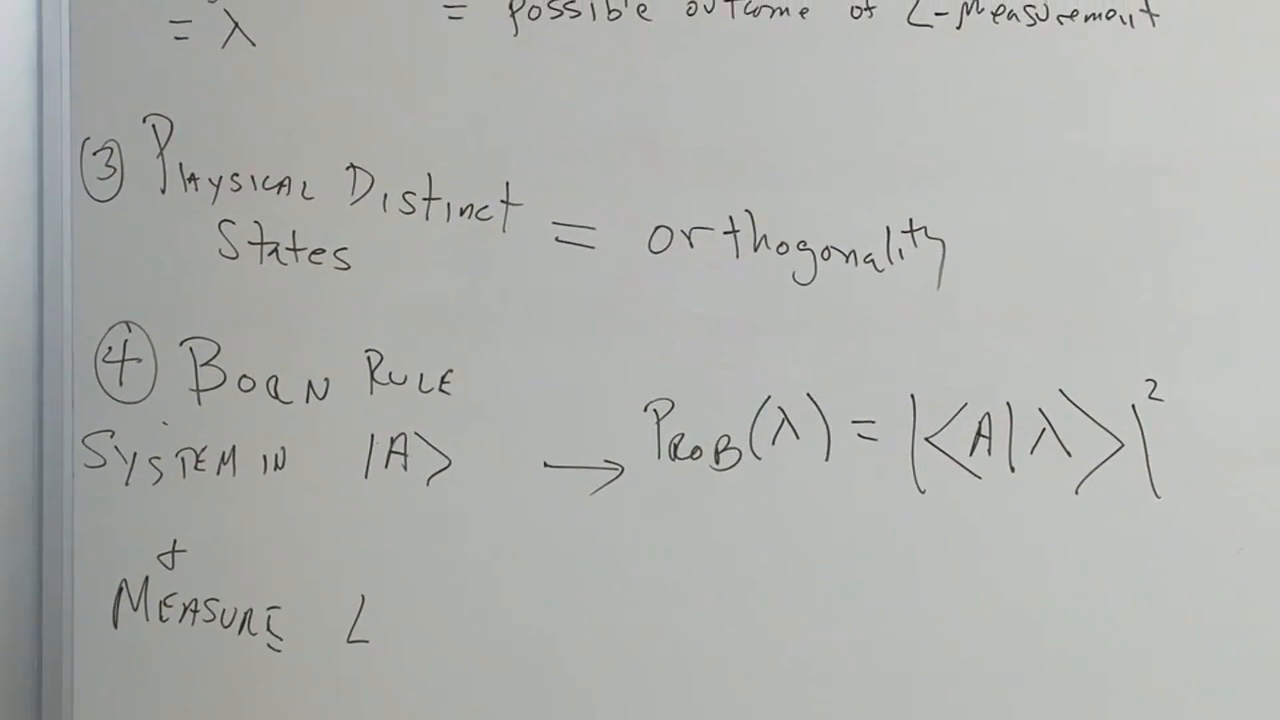
\includegraphics[width=0.86\textwidth]{lecture_04_figure_01.png}
\caption{写在测量原理旁边的玻恩定则：概率是重叠的绝对平方。}
\lectureframe{00:12:40}
\end{figure}

选择 \(L\) 的一组正交归一本征基，并将
\begin{equation}
\ket{A}=\sum_i \alpha_i\ket{\lambda_i},
\qquad
\alpha_i=\braket{\lambda_i}{A}.
\end{equation}
展开。玻恩规则变为
\begin{equation}
P(\lambda_i)=|\alpha_i|^2.
\end{equation}
归一化则给出
\begin{equation}
\sum_i P(\lambda_i)=\sum_i|\alpha_i|^2=1.
\end{equation}
正定性和归一化要求本身并不能推导出玻恩规则，但它们说明了为什么绝对平方如此自然地符合概率论。归根结底，该规则要由实验来检验。

\begin{classroomqa}
\audiencequestion{绝对平方是否也要求所有概率之和为一？}
\lecturerresponse{对于在正交归一基中展开的归一化态，振幅的平方确实之和为一。因此，正定性和归一化与玻恩规则完美契合。哪个陈述在逻辑上更基本，在这里不如它们的相互一致性重要；实验确定了概率规则。}
\end{classroomqa}

\begin{classroomqa}
\audiencequestion{为什么一个本征值，也就是一个数，会被写在 ket 里面？}
\lecturerresponse{记号 \(\ket{\lambda}\) 表示与数值本征值 \(\lambda\) 相关联的本征向量。更拘泥的记号可以引入另一个标签，但过多的指标很快就会使计算变得模糊。ket 符号使数和向量保持区分。}
\end{classroomqa}

\begin{classroomqa}
\audiencequestion{哪个原理将几个可能的结果变成一个实际结果？}
\lecturerresponse{玻恩规则赋予概率。如果制备的态已经是 \(L\) 的本征向量，则其对应结果具有概率一。对于叠加态，会以方程~\eqref{eq:l4-born-rule}中的概率得到某一个结果。相关的态更新或坍缩规则是一个进一步的测量问题；在有了纠缠之后会重新讨论。}
\end{classroomqa}

\subsection{简并结果}

一个本征值可能属于不止一个独立的本征向量。假设
\begin{align}
L\ket{\lambda,1}&=\lambda\ket{\lambda,1},\\
L\ket{\lambda,2}&=\lambda\ket{\lambda,2}.
\end{align}
它们张成空间中的每个线性组合也是本征值为 \(\lambda\) 的本征向量：
\begin{equation}
L\bigl(\alpha\ket{\lambda,1}+\beta\ket{\lambda,2}\bigr)
=
\lambda\bigl(\alpha\ket{\lambda,1}+\beta\ket{\lambda,2}\bigr).
\end{equation}
这种自由度让我们可以在简并本征空间内选择一组正交归一基。如果标签 \(a\) 遍历该基，则数值结果 \(\lambda\) 的概率是其相互排斥的正交通道上的和：
\begin{equation}
P(\lambda)=\sum_a\left|\braket{\lambda,a}{A}\right|^2.
\label{eq:l4-degenerate-born}
\end{equation}
等价地，如果 \(P_\lambda\) 是到整个本征空间的投影算符，那么 \(P(\lambda)=\bra{A}P_\lambda\ket{A}\)。投影算符记号很紧凑；方程~\eqref{eq:l4-degenerate-born}直接展示了概率的相加。

\begin{classroomqa}
\audiencequestion{如果制备的态与几个本征向量都有交叠，或者几个本征向量共享同一本征值，会怎样？}
\lecturerresponse{对于不同的本征值，每个交叠给出其自身结果的概率。对于具有同一本征值的几个正交本征向量，将交叠取平方后相加。如果最初在简并子空间中选择的向量不正交，先将其替换为一组正交归一基；求和后的概率与基无关。}
\end{classroomqa}

\begin{classroomqa}
\audiencequestion{对于一个制备完全未知的自旋，能否得到明确的答案？}
\lecturerresponse{不能从一个任意的样本得到。如果对其制备方式没有限制，就没有单次测量能明确地识别一个未知量子态。制备信息指定了测量可以区分的各种备选。}
\end{classroomqa}

\section{新问题：态如何变化}

前面的原理规定了态和测量。动力学追问的是一个时刻到另一个时刻之间发生了什么。经典类比很有用。一个两态硬币可能在每个时刻都保持不变，也可能交替出现正面、反面、正面、反面。一个六面骰子允许更多更新规则，而连续状态空间允许无穷多个。动力学定律将当前态映射到下一个态。

一个令人满意的经典定律是确定性的且可逆的。不同的态不会合并成一个态，因为如果合并了，现在就不再决定过去。这种信息的保持有时被称为\emph{负第一定律}：它先于更熟悉的守恒定律。

量子版本从一个态向量 \(\ket{\psi(t)}\) 开始，并明确将其视为时间的函数。假设存在单个线性时间演化算符 \(U(t)\)，使得
\begin{equation}
\ket{\psi(t)}=U(t)\ket{\psi(0)}.
\label{eq:l4-time-development}
\end{equation}
同一个 \(U(t)\) 作用于系统的每个初始态。它不是根据输入向量重新选择的，而且其作用是线性的。可以想象更一般的非线性或依赖状态的定律，但它们会迅速与量子力学的概率、因果和复合系统结构相冲突。

\subsection{可逆性保持交叠}

设第二个初始态按同一规律演化：
\begin{equation}
\ket{\phi(t)}=U(t)\ket{\phi(0)}.
\end{equation}
如果两个制备态在初始时刻是可区分的，它们就必须保持可区分。因此
\begin{equation}
\braket{\psi(0)}{\phi(0)}=0
\quad\Longrightarrow\quad
\braket{\psi(t)}{\phi(t)}=0.
\end{equation}

\begin{figure}[htbp]
\centering
\includegraphics[width=0.86\textwidth]{lecture_04_figure_02.png}
\caption{两个态在同一\(U(t)\)下演化；初始的正交性保持为正交性。}
\lectureframe{00:34:43}
\end{figure}

保持归一化态和正交性，已足以保持所有内积。为看清其机制，将两个任意矢量按正交归一基展开。基矢量在演化下仍保持正交归一，因此系数在每一时刻都重构出相同的重叠：
\begin{equation}
\braket{\psi(t)}{\phi(t)}=\braket{\psi(0)}{\phi(0)}.
\label{eq:l4-overlap-conservation}
\end{equation}
因此，不仅完全可区分性，而且两个态之间相似程度的全部内容都守恒。

与式~\eqref{eq:l4-time-development}对应的左矢由厄米共轭得到：
\begin{equation}
\bra{\psi(t)}=\bra{\psi(0)}U^\dagger(t).
\end{equation}
将左矢和右矢的演化代入式~\eqref{eq:l4-overlap-conservation}，得到
\begin{equation}
\bra{\psi(0)}U^\dagger(t)U(t)\ket{\phi(0)}
=
\braket{\psi(0)}{\phi(0)}
\end{equation}
对每一对初始矢量都成立。如果一个算符在每一对矢量之间的矩阵元都与恒等算符相同，那么它就是恒等算符。因此
\begin{equation}
U^\dagger(t)U(t)=I.
\label{eq:l4-unitarity}
\end{equation}
满足式~\eqref{eq:l4-unitarity}的算符是\emph{幺正的}。在有限维情形下，
\begin{equation}
U^\dagger(t)=U^{-1}(t),
\end{equation}
因此演化可以反向进行。

\begin{classroomqa}
\audiencequestion{这里大写和小写的\(\Phi\)表示不同种类的态吗？}
\lecturerresponse{不是。那只是书写不一致。我们一致地使用\(\ket{\phi}\)；数学上区分态靠的是它们的标签和取值，而不是偶然的大小写。}
\end{classroomqa}

\begin{classroomqa}
\audiencequestion{能否把\(U^\dagger U=I\)理解为其中一个因子是另一个的逆？}
\lecturerresponse{可以。幺正算符的逆为\(U^{-1}=U^\dagger\)。这正是可逆、保重叠演化的代数表述。}
\end{classroomqa}

\section{无穷小时间与哈密顿量}

在零经过时间下没有任何变化，所以\(U(0)=I\)。对于非常小的时间间隔\(\epsilon\)，\(U(\epsilon)\)必须接近恒等算符。在暂时取\(\hbar=1\)的单位制下，写出
\begin{equation}
U(\epsilon)=I-i\epsilon H+O(\epsilon^2).
\label{eq:l4-small-u}
\end{equation}
负号和因子\(i\)起初只是约定；在不知道\(H\)的情况下，它们可以被吸收进它的定义中。它们的有用性在施加幺正性时显现出来。厄米共轭给出
\begin{equation}
U^\dagger(\epsilon)=I+i\epsilon H^\dagger+O(\epsilon^2).
\end{equation}
于是
\begin{align}
I
&=U^\dagger(\epsilon)U(\epsilon)\\
&=\bigl(I+i\epsilon H^\dagger\bigr)
  \bigl(I-i\epsilon H\bigr)+O(\epsilon^2)\\
&=I+i\epsilon(H^\dagger-H)+O(\epsilon^2).
\end{align}
一阶项必须为零：
\begin{equation}
H^\dagger=H.
\label{eq:l4-h-hermitian}
\end{equation}

\begin{figure}[htbp]
\centering
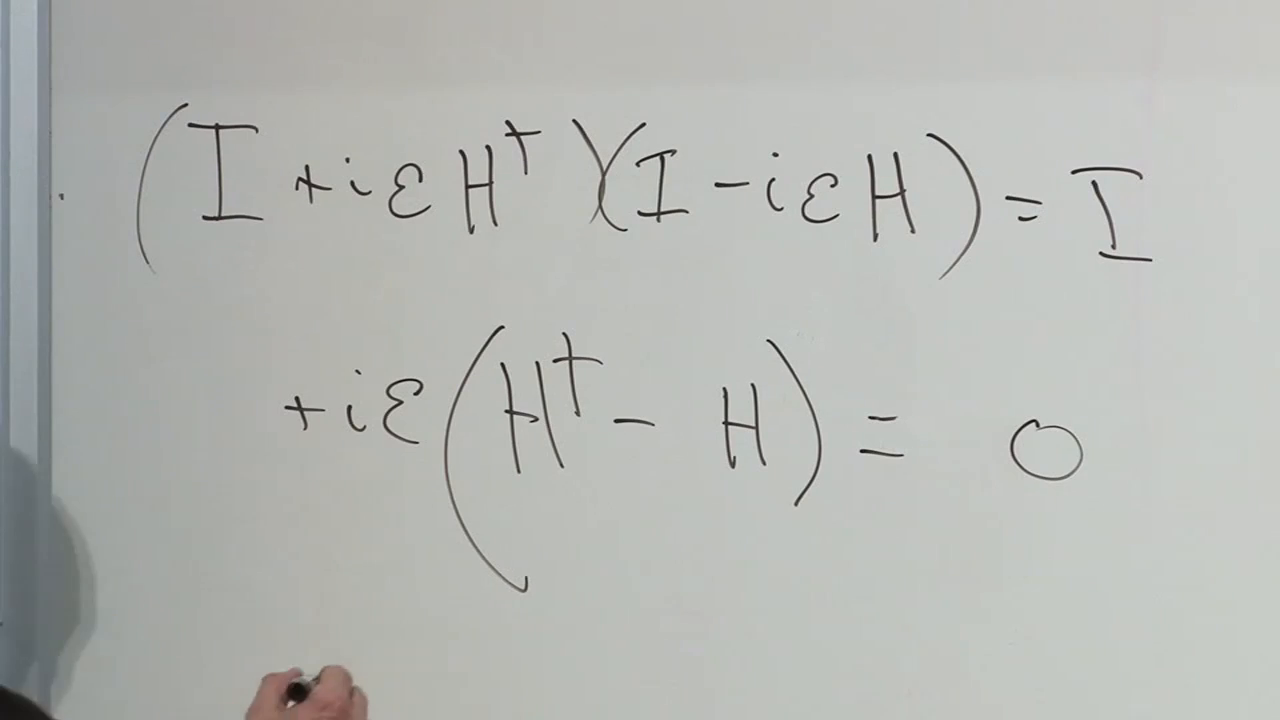
\includegraphics[width=0.86\textwidth]{lecture_04_figure_03.png}
\caption{一阶幺正性计算迫使无穷小生成元为厄米的。}
\lectureframe{00:43:38}
\end{figure}

字母\(H\)并不代表厄米，而代表\emph{哈密顿量}。由于它是厄米的，它代表一个可观测量。它被等同于能量，而在更结构性的意义上，被等同于时间平移的生成元。这种等同并不止于一个名称：在具有已知经典极限的系统中，量子\(H\)必须再现经典哈密顿量的动力学。对称性、自由度、物理判断，最终还有实验，决定哪一个厄米算符是某个特定系统的哈密顿量。

\begin{classroomqa}
\audiencequestion{任何厄米算符都可以用作\(H\)吗？是什么选出了实际的那一个？}
\lecturerresponse{到目前为止的推导允许系统希尔伯特空间上的任何厄米算符。物理则选出由该系统自由度构建的那一个。对于自旋，它必须由自旋算符和外场构成。对称性和已知相互作用缩小了可能性；实验确定剩余的常数，有时还确定形式本身。}
\end{classroomqa}

哈密顿量可以显式依赖于时间。一个电流正在被改变的磁场提供了一个简单例子。如果外部参数与时间无关，那么\(H\)没有显式时间依赖；这就是时间平移不变性。如果参数随时间被驱动，能量就不必守恒。

\begin{classroomqa}
\audiencequestion{在小时间展开中，\(H\)是一个常数，还是应当写成\(H(0)\)？}
\lecturerresponse{对于与时间无关的问题，\(H\)在每一时刻都是同一个算符。更一般地，从时刻\(t\)开始的局部步长包含\(H(t)\)。这里的推导先处理时间平移不变的情形，随后说明显式时间依赖如何改变能量守恒。}
\end{classroomqa}

\section{含时Schr\"odinger方程}

将式~\eqref{eq:l4-small-u}作用于该态：
\begin{equation}
\ket{\psi(\epsilon)}=(I-i\epsilon H)\ket{\psi(0)}+O(\epsilon^2).
\end{equation}
整理并除以\(\epsilon\)，
\begin{equation}
\frac{\ket{\psi(\epsilon)}-\ket{\psi(0)}}{\epsilon}
=-iH\ket{\psi(0)}+O(\epsilon).
\label{eq:l4-difference-quotient}
\end{equation}

\begin{figure}[htbp]
\centering
\includegraphics[width=0.86\textwidth]{lecture_04_figure_04.png}
\caption{将无穷小态更新整理成矢量值差商。}
\lectureframe{00:51:42}
\end{figure}

对矢量求导并没有什么特别神秘之处。两个矢量可以相减，它们的差可以除以一个数，而极限定义了另一个矢量。上面称为零的那个参考时刻可以是任意一个瞬间。因此取\(\epsilon\to0\)就得到
\begin{equation}
\boxed{\frac{d}{dt}\ket{\psi(t)}=-iH\ket{\psi(t)}}
\qquad(\hbar=1).
\label{eq:l4-schrodinger-natural}
\end{equation}

\begin{figure}[htbp]
\centering
\includegraphics[width=0.86\textwidth]{lecture_04_figure_05.png}
\caption{黑板上完成的推导最终归结为方框中的含时Schr\"odinger方程。}
\lectureframe{00:56:11}
\end{figure}

这就是广义的含时Schr\"odinger方程。我们熟悉的关于粒子波函数的微分方程，只是这个抽象态矢量方程的一种表示。要使用它，必须知道\(H\)以及初始态。

对于有限区间，求解该微分方程。当\(H\)不随时间变化时，反复复合无穷小步骤给出
\begin{equation}
U(t)=e^{-iHt}
\qquad(\hbar=1),
\end{equation}
这正是把所有小步骤复合起来的精确版本。含时哈密顿量需要时间排序，这一精细之处我们留待以后讨论。

\begin{classroomqa}
\audiencequestion{上述展开使用了无穷小区间。那么长时间之后的状态由什么决定？}
\lecturerresponse{反复施加无穷小更新，或者等价地求解微分方程。对于不随时间变化的\(H\)，这些小步骤的乘积成为\(e^{-iHt/\hbar}\)。}
\end{classroomqa}

\subsection{恢复普朗克常数}

前面的方程使用了\(\hbar=1\)的单位制。量纲分析表明\(\hbar\)应当出现在哪里。导数具有时间的倒数量纲，而\(H\)具有能量的量纲。由于\(\hbar\)具有能量乘时间的量纲，
\begin{equation}
\boxed{i\hbar\frac{d}{dt}\ket{\psi(t)}=H\ket{\psi(t)}}.
\label{eq:l4-schrodinger}
\end{equation}
等价地，无穷小算符为\(U(\epsilon)=I-i\epsilon H/\hbar+O(\epsilon^2)\)，而不含时的有限时间演化为\(U(t)=e^{-iHt/\hbar}\)。

\begin{classroomqa}
\audiencequestion{普朗克常数究竟出现在哪里？}
\lecturerresponse{普朗克常数以下面两种等价形式之一出现
\begin{align*}
i\hbar\,\partial_t\ket{\psi}&=H\ket{\psi},\\
\partial_t\ket{\psi}&=-\frac{i}{\hbar}H\ket{\psi}.
\end{align*}
两者的量纲都匹配，因为\(\hbar\)具有能量乘时间的单位。}
\end{classroomqa}

态按照方程~\eqref{eq:l4-schrodinger}确定性地演化；测量结果仍然是统计性的，因为它们是由玻恩定则从连续变化的态中抽样得到的。

\begin{classroomqa}
\audiencequestion{这一推导是否依赖于可逆性，它又如何能在扰动态的测量下继续成立？}
\lecturerresponse{它依赖于线性演化和内积守恒。该方程描述的是一个孤立系统。测量仪器相互作用强到足以成为物理系统的一部分，因而不能被忽略。系统与仪器的组合必须用量子力学处理；它们的纠缠正是分析测量之前必须理解的东西。}
\end{classroomqa}

\section{期望值意味着平均}

为了将量子动力学与经典方程相比较，我们需要可观测量的平均值。标准名称\emph{期望值}可能引起误解。对于一个只取\(+1\)和\(-1\)的公平变量，平均值是零，尽管从未观测到零。一个对称分布甚至可以在其均值附近的整个邻域内都为零。对于某些光滑的单峰分布，均值、中位数和众数重合，但一般而言并非如此。

如果\(L\)能以概率\(P(\lambda_i)\)返回数值\(\lambda_i\)，则定义
\begin{equation}
\overline{\lambda}=\sum_i\lambda_iP(\lambda_i).
\label{eq:l4-probability-average}
\end{equation}
这是分布的一阶矩，而不是对单次试验结果的承诺。

\begin{classroomqa}
\audiencequestion{最频繁出现的值不才是人们应当期待的吗？}
\lecturerresponse{最频繁出现的值是众数；加权平均是均值。对于一个简单的窄分布，它们可能重合，但一个双峰分布的均值可以落在概率基本为零的区域。期望一词指的是数学均值，而不一定是最可能的单一结果。}
\end{classroomqa}

重复试验将数学均值与数据联系起来。在通常的独立性和有限矩假设下，大数定律陈述的是样本平均值的概率收敛。它们并不保证每一个有限序列都接近均值；一段极其漫长的相同自旋结果序列仍然是可能的，只是概率很小。这正是同一个统计上的微妙之处，它使热力学第二定律不至于成为一条毫无例外的微观禁令。

\begin{classroomqa}
\audiencequestion{如果一次公平的自旋实验碰巧连续给出一百万个上，它的平均值真的是上吗？}
\lecturerresponse{那一次特定实验的样本平均值确实是上。理论期望值仍然是零。随着独立试验次数增加，样本平均值以高概率趋近理论平均值，但概率论从不排除每一个例外的有限序列。}
\end{classroomqa}

\subsection{算符夹心}

将归一化态在\(L\)的正交归一本征基中展开：
\begin{equation}
\ket{A}=\sum_i\alpha_i\ket{\lambda_i},
\qquad
\bra{A}=\sum_j\alpha_j^*\bra{\lambda_j}.
\end{equation}
玻恩定则与式~\eqref{eq:l4-probability-average}给出
\begin{equation}
\overline{\lambda}=\sum_i\lambda_i|\alpha_i|^2.
\end{equation}
现在计算
\begin{align}
\bra{A}L\ket{A}
&=\sum_{i,j}\alpha_j^*\alpha_i
  \bra{\lambda_j}L\ket{\lambda_i}\\
&=\sum_{i,j}\alpha_j^*\alpha_i\lambda_i
  \braket{\lambda_j}{\lambda_i}\\
&=\sum_i\lambda_i|\alpha_i|^2.
\end{align}
由于\(\braket{\lambda_j}{\lambda_i}=\delta_{ji}\)，双重求和坍缩。因此
\begin{equation}
\boxed{\expect{L}_A=\bra{A}L\ket{A}}.
\label{eq:l4-expectation-sandwich}
\end{equation}

\begin{figure}[htbp]
\centering
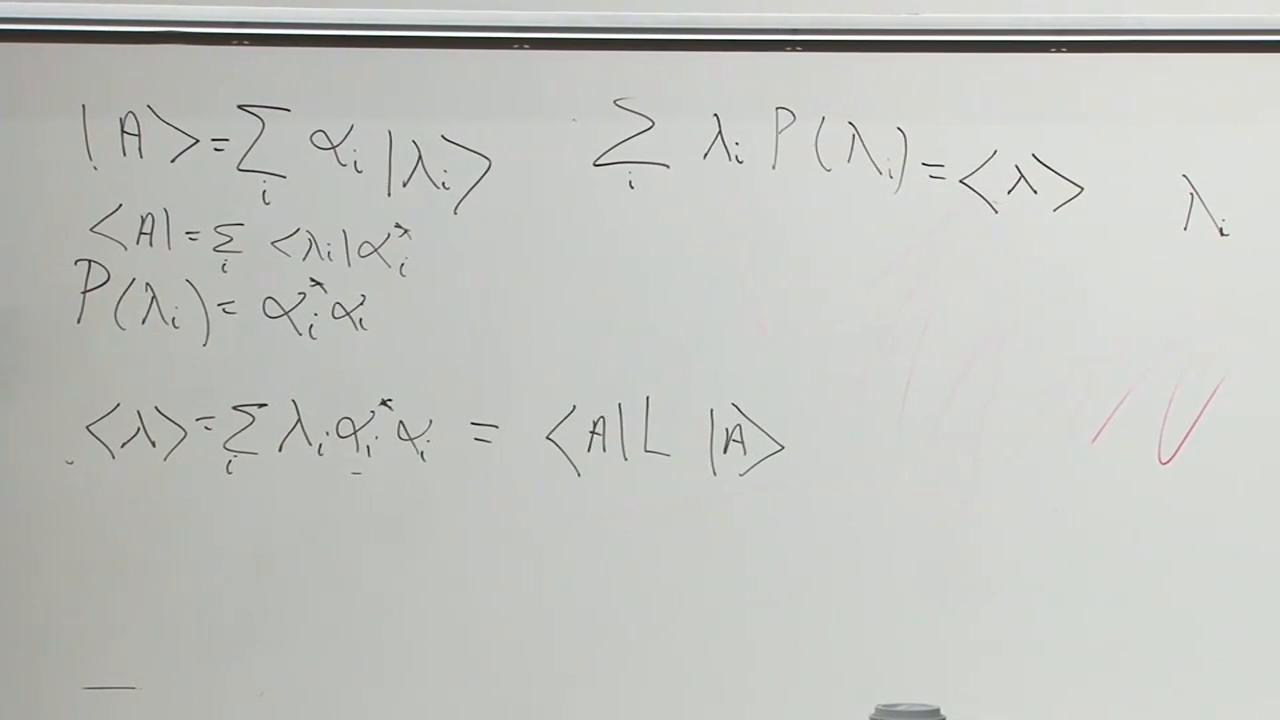
\includegraphics[width=0.86\textwidth]{lecture_04_figure_06.png}
\caption{本征基展开将概率平均归结为算符夹心\(\bra{A}L\ket{A}\)。}
\lectureframe{01:11:50}
\end{figure}

尖括号和上划线都将用于表示平均值。当态演化时，
\begin{equation}
\expect{L}_t=\bra{\psi(t)}L\ket{\psi(t)}.
\end{equation}
下标只是提醒我们，态因而平均值依赖于时间。在当前的Schr\"odinger绘景讨论中，除非明确说明存在显式时间依赖，\(L\)本身是固定的。

\begin{classroomqa}
\audiencequestion{\(t\)应该写在括号外面吗，上划线表示样本平均值吗？}
\lecturerresponse{两种记号都可以加注以显示时间依赖，但标准的量子记号是\(\expect{L}_t\)，或者简写为\(\expect{L}\)，时间由\(\ket{\psi(t)}\)理解。这里上划线表示理论概率平均值，即一阶矩\(\sum_i\lambda_iP(\lambda_i)\)，并非特指有限数据的样本平均值。}
\end{classroomqa}

\section{平均值如何演化}

用乘积法则对夹心求导：
\begin{equation}
\frac{d}{dt}\expect{L}
=
\left(\frac{d}{dt}\bra{\psi}\right)L\ket{\psi}
+
\bra{\psi}L\left(\frac{d}{dt}\ket{\psi}\right).
\label{eq:l4-product-derivative}
\end{equation}
在\(\hbar=1\)单位下，右矢方程及其厄米共轭为
\begin{align}
\frac{d}{dt}\ket{\psi}&=-iH\ket{\psi},\\
\frac{d}{dt}\bra{\psi}&=+i\bra{\psi}H.
\end{align}
\(i\)的符号在复共轭下改变，且\(H^\dagger=H\)。代入式~\eqref{eq:l4-product-derivative}给出
\begin{align}
\frac{d}{dt}\expect{L}
&=i\bra{\psi}HL\ket{\psi}
-i\bra{\psi}LH\ket{\psi}\\
&=i\bra{\psi}(HL-LH)\ket{\psi}.
\end{align}

算符不必对易。它们的顺序很重要，正如矩阵的顺序很重要。定义
\begin{equation}
[H,L]=HL-LH.
\end{equation}
则
\begin{equation}
\boxed{\frac{d}{dt}\expect{L}=i\expect{[H,L]}}
\qquad(\hbar=1).
\label{eq:l4-average-evolution-natural}
\end{equation}

\begin{figure}[htbp]
\centering
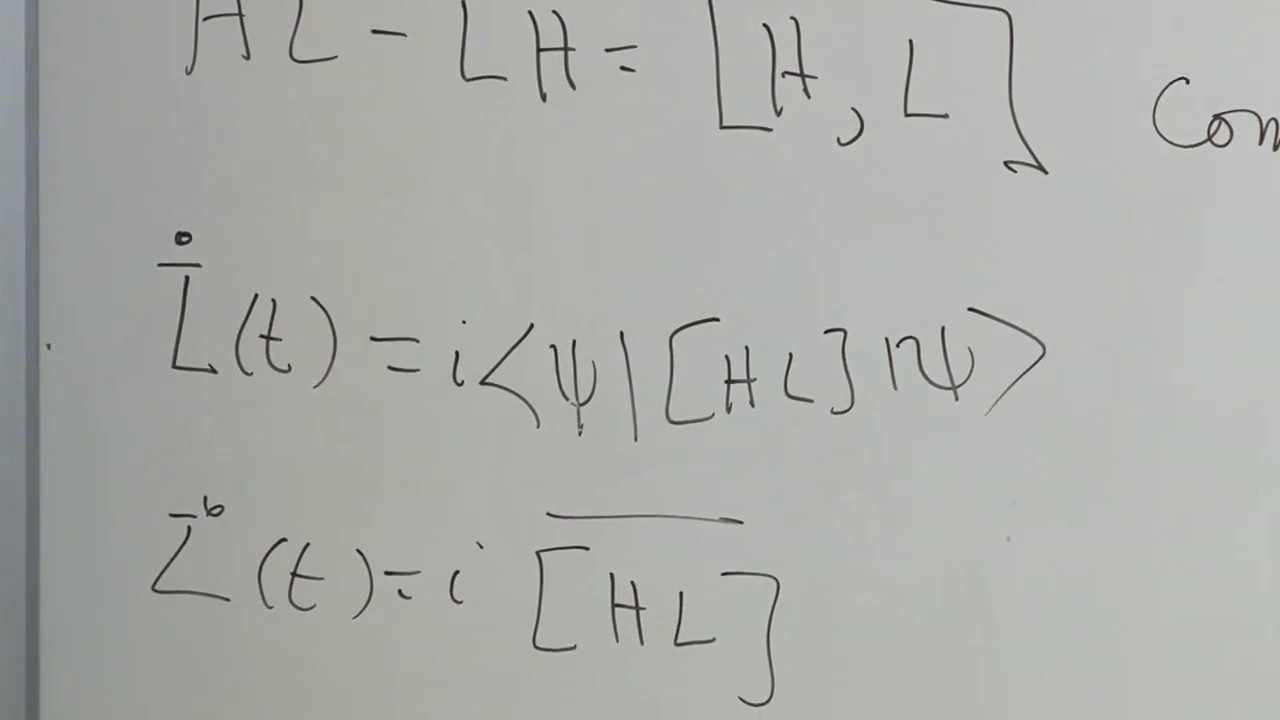
\includegraphics[width=0.86\textwidth]{lecture_04_figure_07.png}
\caption{平均值的导数由对易子的期望值决定。}
\lectureframe{01:22:22}
\end{figure}

恢复量纲后，
\begin{equation}
\boxed{\frac{d}{dt}\expect{L}
=\frac{i}{\hbar}\expect{[H,L]}
=-\frac{i}{\hbar}\expect{[L,H]}}.
\label{eq:l4-average-evolution}
\end{equation}
如果\(L\)本身显式依赖于时间，一般方程包含附加项\(\expect{\partial L/\partial t}\)。这里\(L\)是固定的。

\begin{classroomqa}
\audiencequestion{对易子方程中的符号真的是正\(i\)吗？}
\lecturerresponse{是的，当\([H,L]=HL-LH\)时，结果为\(+(i/\hbar)\expect{[H,L]}\)。反转对易子会反转其符号，给出等价形式\(-(i/\hbar)\expect{[L,H]}\)。}
\end{classroomqa}

\begin{classroomqa}
\audiencequestion{左矢方程是通过复共轭还是厄米共轭得到的，为什么导数留在左边？}
\lecturerresponse{是厄米共轭。右矢的导数是右矢，该导数的对偶是对应左矢的导数。可以直接从差商看出这一点：左矢的差是左矢，正如右矢的差是右矢。时间在这里是参数，不是必须反转顺序的算符。}
\end{classroomqa}

\section{经典影子}

在经典哈密顿力学中，一个无显式时间依赖的相空间函数\(L(q,p)\)满足
\begin{equation}
\frac{dL}{dt}=\{L,H\}_{\mathrm{PB}},
\label{eq:l4-poisson-evolution}
\end{equation}
其中\(\{\cdot,\cdot\}_{\mathrm{PB}}\)是泊松括号。将此与式~\eqref{eq:l4-average-evolution}比较。两个括号都是反对称的：
\begin{align}
\{L,H\}_{\mathrm{PB}}&=-\{H,L\}_{\mathrm{PB}},\\
[L,H]&=-[H,L].
\end{align}
两者也都作为乘积上的导数作用：
\begin{align}
\{LM,H\}_{\mathrm{PB}}
&=\{L,H\}_{\mathrm{PB}}M+L\{M,H\}_{\mathrm{PB}},\\
[LM,H]
&=L[M,H]+[L,H]M.
\label{eq:l4-commutator-product}
\end{align}
对易子恒等式通过加上并减去\(LHM\)得到：
\begin{align}
LMH-HLM
&=(LMH-LHM)\\
&\quad +(LHM-HLM)\\
&=L(MH-HM)\\
&\quad +(LH-HL)M.
\end{align}

这种平行性提示了对应关系
\begin{equation}
[A,B]
\quad\longleftrightarrow\quad
i\hbar\{A,B\}_{\mathrm{PB}},
\label{eq:l4-dirac-correspondence}
\end{equation}
或等价地
\begin{equation}
\{A,B\}_{\mathrm{PB}}
\quad\longleftrightarrow\quad
-\frac{i}{\hbar}[A,B].
\end{equation}

\begin{figure}[htbp]
\centering
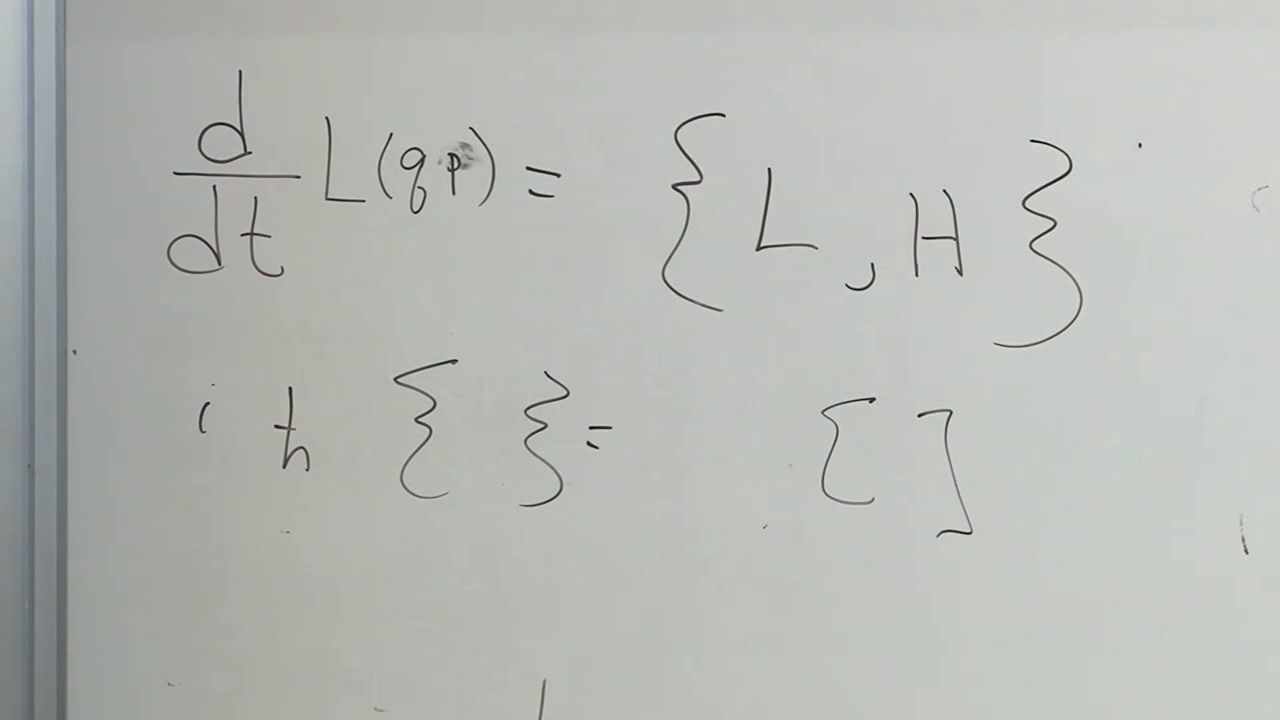
\includegraphics[width=0.86\textwidth]{lecture_04_figure_08.png}
\caption{经典泊松括号方程与量子对易子对应关系，其中\(\hbar\)已恢复。}
\lectureframe{01:32:32}
\end{figure}

狄拉克认识到这一联系，并将其用作进入量子力学的途径。然而必须将其作为对应关系来处理，而不是普遍替换规则：可能出现算符排序歧义，并且经典极限必须从量子动力学推导出来。从概念上讲，量子力学是第一位的；经典力学是其在适当态和尺度下的近似。对易子先于泊松括号，尽管历史类比有助于我们发现这一关系。

\begin{classroomqa}
\audiencequestion{为什么把\(H\)称为能量，又为什么在引入对称性原理之前就推断能量守恒？}
\lecturerresponse{在这个阶段，\(H\)严格地说是时间平移的厄米生成元。把它称为能量是一种物理上的认定，必须在已知经典极限的地方加以检验。对于处于适当状态的大尺度或重系统，量子平均值必须遵循经典方程，而量子\(H\)必须与经典哈密顿量相联系。下面的守恒陈述假定该生成元没有显式的时间依赖。}
\end{classroomqa}

\section{平均能量守恒}

取方程~\eqref{eq:l4-average-evolution}中的\(L=H\)，哈密顿量不依赖于时间：
\begin{equation}
\frac{d}{dt}\expect{H}
=\frac{i}{\hbar}\expect{[H,H]}.
\end{equation}
任何算符都与自身对易，
\begin{equation}
[H,H]=HH-HH=0,
\end{equation}
因此
\begin{equation}
\boxed{\frac{d}{dt}\expect{H}=0}.
\label{eq:l4-energy-conservation}
\end{equation}

\begin{figure}[htbp]
\centering
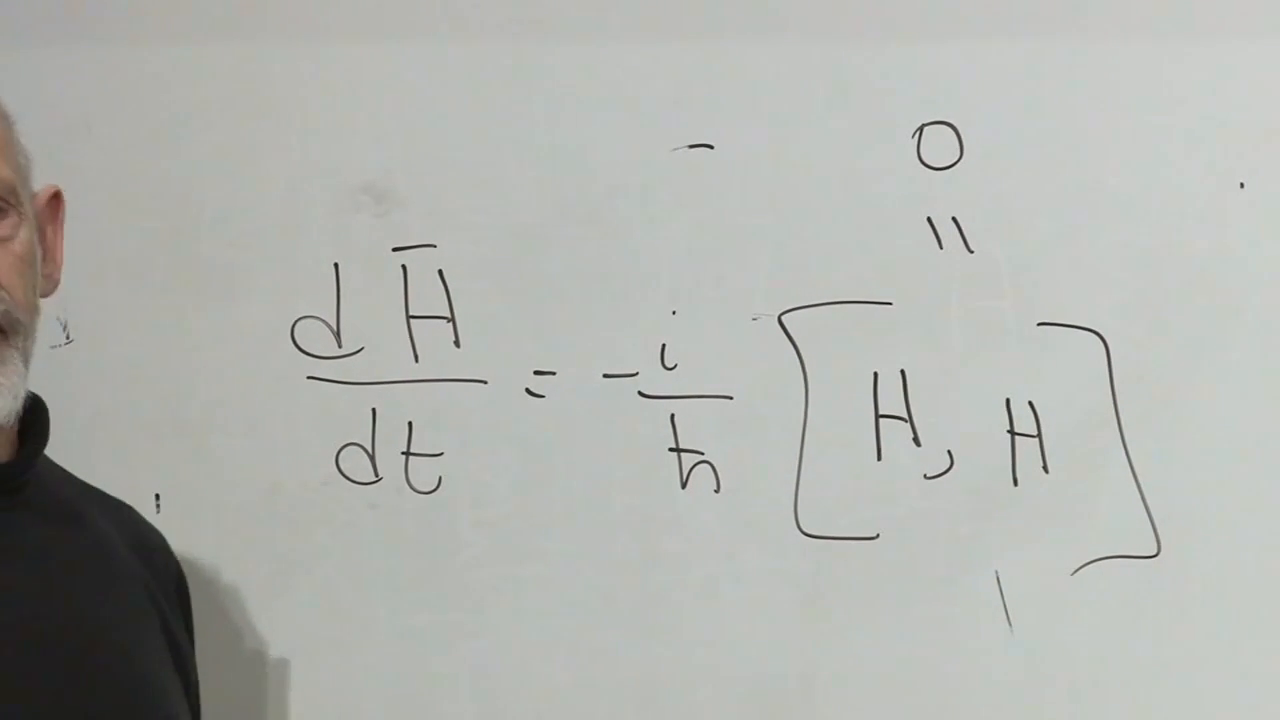
\includegraphics[width=0.86\textwidth]{lecture_04_figure_09.png}
\caption{平均能量守恒立即成立，因为哈密顿量与自身对易。}
\lectureframe{01:39:30}
\end{figure}

这证明了一个刻意保持谨慎的陈述：平均能量是常数。关于整个能量分布的更强陈述将由同样的动力学得出。如果\(H\)显式依赖于时间，额外的显式导数就不必为零，受驱动的系统可以与其参数发生变化的任何东西交换能量。

还有两条线索尚未了结。任意轴自旋概率的计算仍在等待，而状态更新问题尚未推导出来。在干预之间，孤立状态幺正演化。在测量期间，系统与仪器相互作用并发生纠缠。

\begin{classroomqa}
\audiencequestion{之前承诺的沿任意轴测量自旋的概率怎么样了？}
\lecturerresponse{一般动力学占用了可用的时间。自旋计算仍是下一个具体的应用，将在这一结构框架之后继续。}
\end{classroomqa}

\begin{classroomqa}
\audiencequestion{如果没有坍缩公设，这些公设怎么能是完备的？}
\lecturerresponse{目前坍缩只是暂行的说法。一次测量建立了系统与仪器之间的纠缠。在复合系统和纠缠得到展开之前，测量过程无法被诚实地建模。这是下一个概念步骤。}
\end{classroomqa}
